% Chapter 

\chapter{Conclusion} % Main chapter title

\label{Conclusion} % For referencing the chapter elsewhere, use \ref{Chapter1} 

% \lhead{Chapter 1. \emph{Introduction}} % This is for the header on each page - perhaps a shortened title

\graphicspath{{./Pictures/}}

%----------------------------------------------------------------------------------------

The present thesis addresses late nuclear maturation steps of the non-enveloped parvovirus minute virus of mice (MVM), which ultimately initiate the process of nuclear export and egress of the virion progeny. The current knowledge about nuclear maturation, export, and egress of non-enveloped viruses is limited. Although non-enveloped viruses have always been thought to being passively released by virus-induced cytolysis, growing evidence suggests an active mechanism for the egress of progeny virions.   

Anion-exchange chromatography (AEX) was applied to separate intracellular virus populations displaying different protein surface electrostatics. Apart from empty capsids (EC), two well defined DNA-containing populations were separated based on their net surface electrostatics. The full capsid (FC) populations, referred to as FC-P\textsubscript{1} and FC-P\textsubscript{2}, differed in the conformation of their N-termini of the viral capsid protein VP2 (N-VP2), as well as in their surface phosphorylations. Nuclear export was observed only for the FC-P\textsubscript{2} population, resulting in distinct subcellular localization leading to a segregation of both FC populations. Thus, an active mechanism for virus egress was confirmed. While N-VP2 was not involved in the active nuclear export of MVM, the phosphorylations were strictly associated to nuclear export. During their life cycle, karyophilic viruses encounter a paradoxical situation. Early in infection, the virus has to enter the nucleus where it usurps the replication machinery of the host cell. Following assembly and DNA-packaging, progeny virions are exported from the nucleus to egress the infected cell. In order to fulfill a complete infection cycle, the virus needs to rearrange its capsid surface to switch from an import mode to an export mode and vice versa. Figure~\ref{Scheme}, p.~\pageref{Scheme} summarizes the spatially and temporally controlled modifications in capsid surface phosphorylation providing nuclear import and export potential required to complete the life cycle of a karyophilic virus. Significantly, the surface phosphorylations of the FC-P\textsubscript{2} population were removed during endocytic trafficking of incoming virions. The FC-P\textsubscript{2} population adopted the surface phosphorylation pattern of the FC-P\textsubscript{1} population. Acidic phosphatases hydrolyzed the corresponding phosphorylations. The endocytic dephosphorylation was sensitive to basification of the endosomes by lysosomotropic compounds.

N-VP2 was shown to be dispensable for this step. The phosphoserine-rich N-VP2 was demonstrated to mediate the rearrangement of the cytoskeleton late in infection. N-VP2 defective mutants showed prolonged endocytic VP2 processing and thus delayed nuclear targeting.       
   







\begin{figure}[H]
\centering
  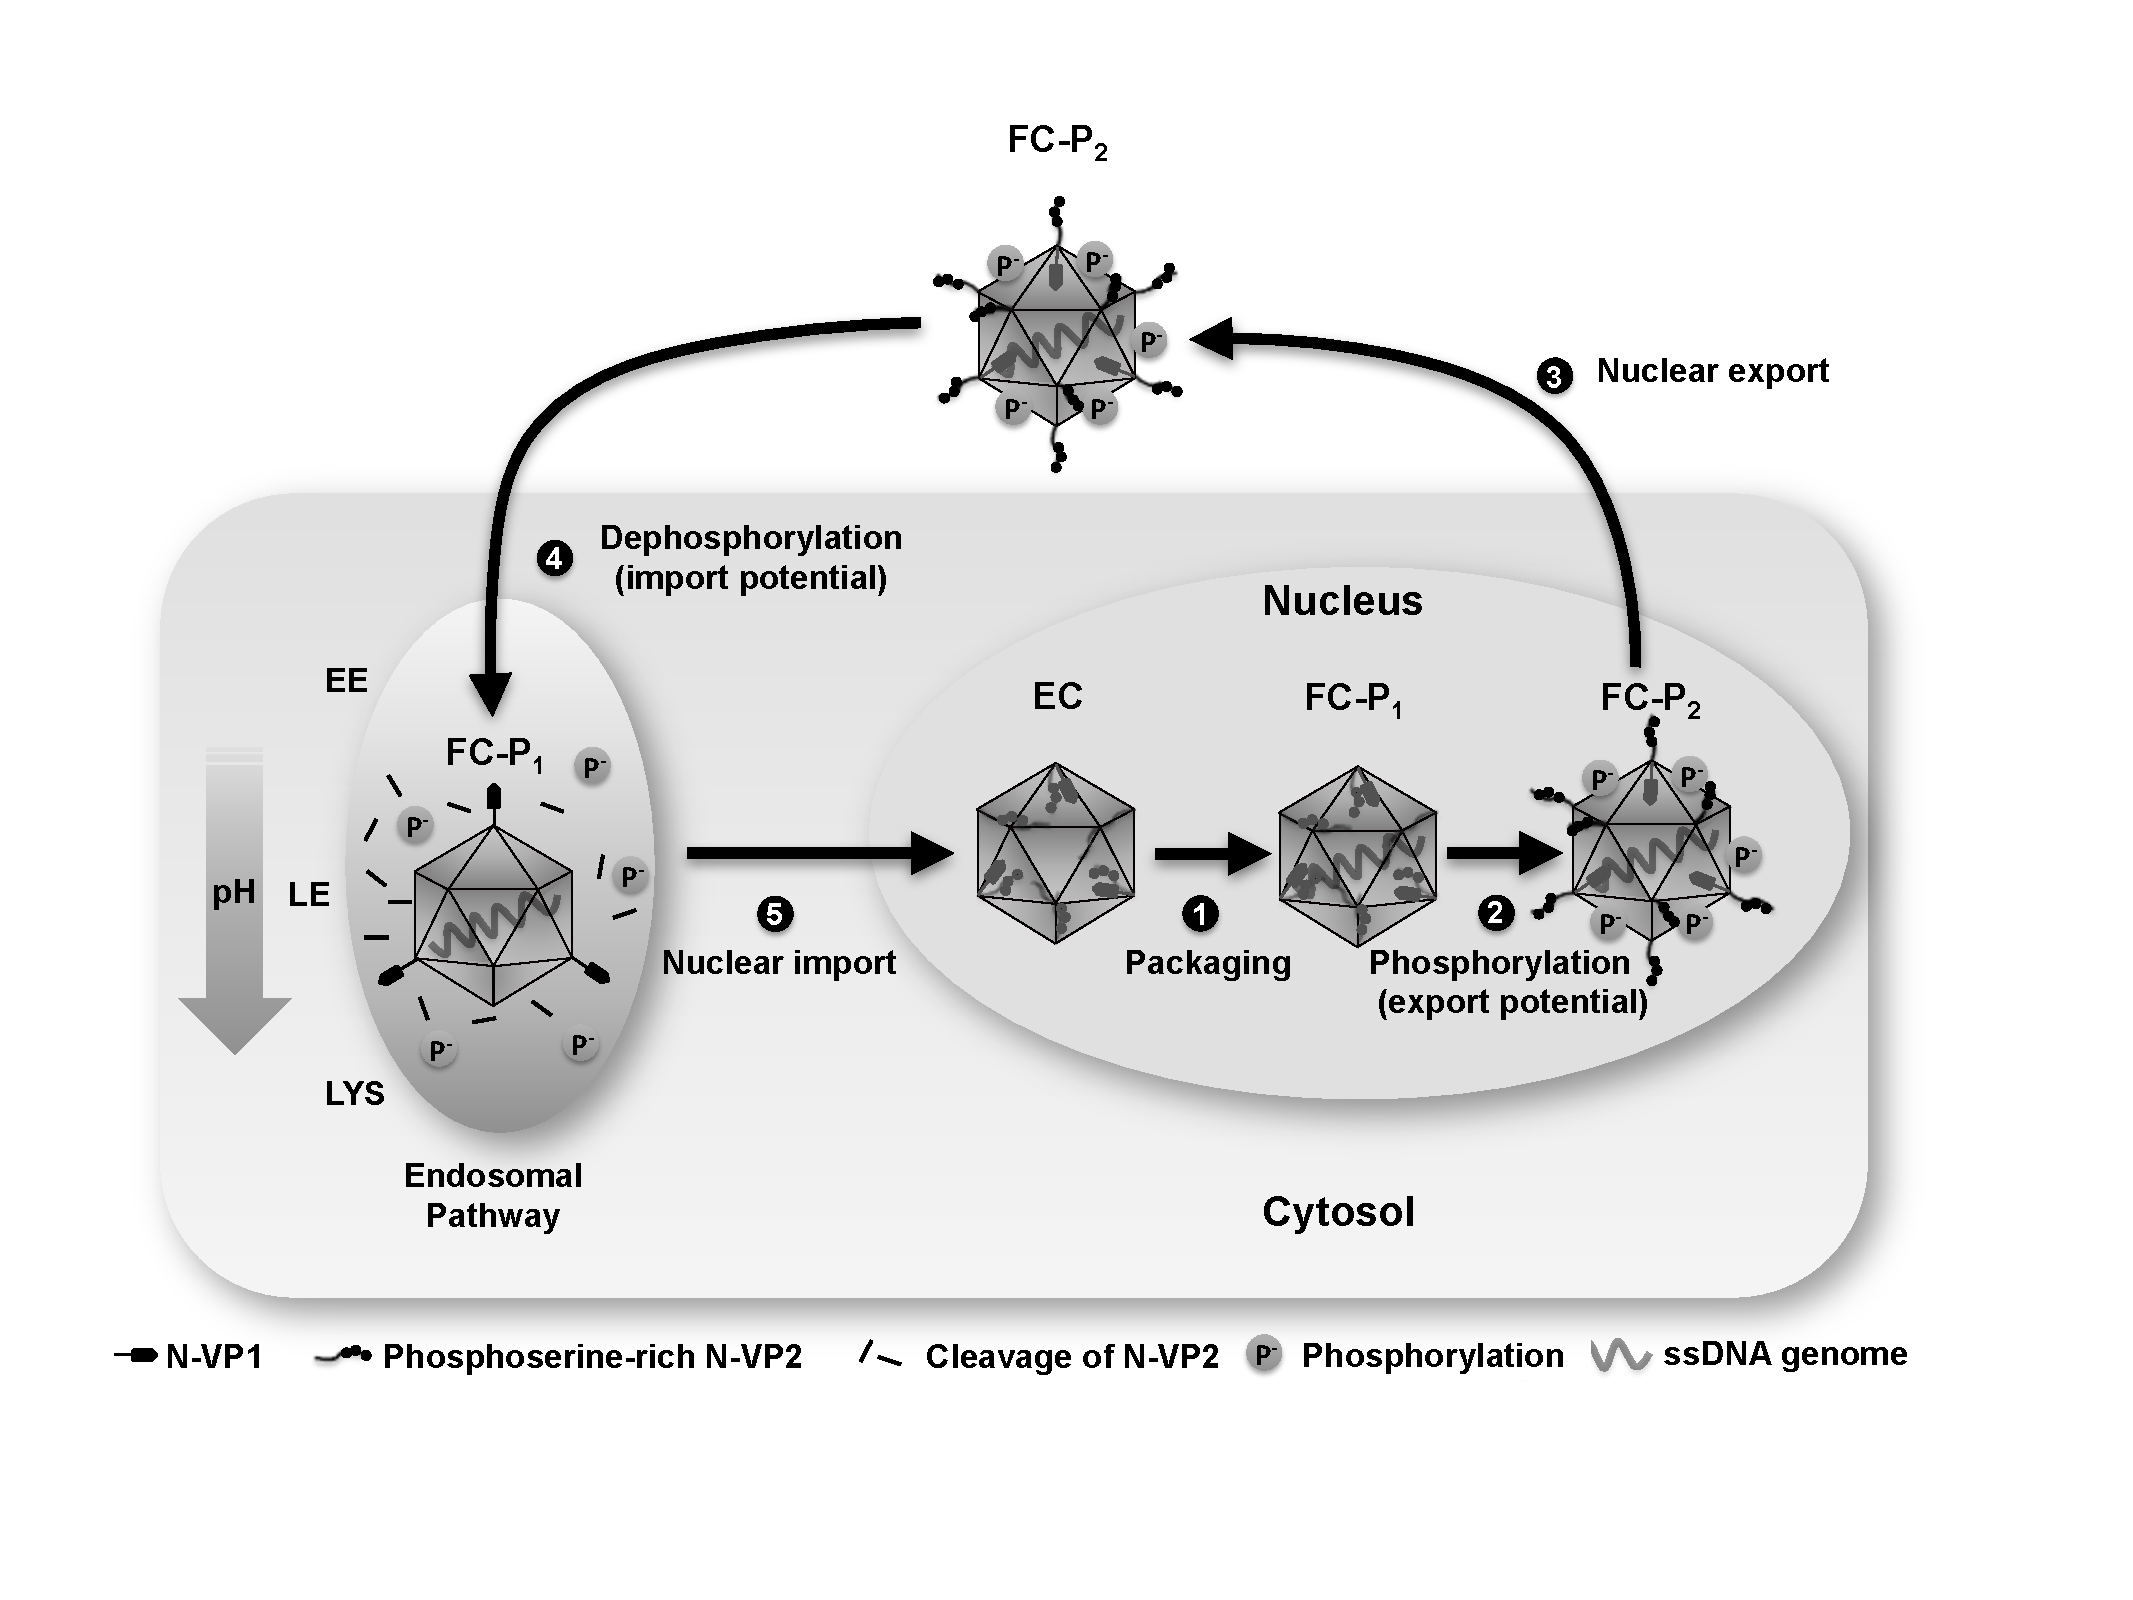
\includegraphics[width=\textwidth]{Conclusion}
  \caption[Schematic representation of nuclear import and export of MVM.]
   {Surface phosphorylations play a pivotal role in determining the nuclear export of MVM. The virus life cycle is summarized in 5 steps. Following self-assembly of the structural proteins, the empty capsids (EC) are filled with a ssDNA genome, leading to the generation of FC-P\textsubscript{1} virions (step 1). FC-P\textsubscript{1} particles are phosphorylated by a nuclear kinase, resulting in the accumulation of FC-P\textsubscript{2} virion progeny (step 2). FC-P\textsubscript{2} virions are exported from the nucleus of infected cells and egress the host cell (step 3). During entry, export competent FC-P\textsubscript{2} virions become dephosphorylated by acidic phosphatases, adopting the FC-P\textsubscript{1} surface electrostatics (step 4). Infectious incoming virions escape the endosomal pathway and are imported into the nucleus (step 5). The most important capsid elements involved in the viral life cycle are explained below the representation.} 
\label{Scheme}
\end{figure}















% Recent research in our lab focused on dynamics and structural rearrangements on the surface of parvovirus capsids during the first stages of an infection. The studies were conducted on both parvoviruses B19V and MVM. For the latter model virus, three major pH-dependent structural capsid rearrangements were observed \textit{in vivo}. These include the proteolytic digestion of N-VP2, the externalization of N-VP1 through the cylindrical 5-fold channel, and the externalization of viral DNA which remained associated to the capsid (see Section~\ref{Rearrangements}, p.~\pageref{Rearrangements}) \cite{pmid16379002}. To date, neither the triggers causing these endosomal rearrangements nor their purpose have been elucidated in detail. B19V has been shown to undergo conformational changes upon binding to its primary attachment receptor globoside (Gb4Cer), also referred to as erythrocyte P antigen. Binding to the receptor triggers the externalization of VP1u, the highly immunogenic N-terminus of the minor structural capsid protein VP1 \cite{pmid20826697}. VP1u has been shown to be the key determinant for the extraordinarily restricted B19V tropism \cite{pmid24067971}. Most recent results obtained in our lab indicate that B19V undergoes phosphorylation events during cytoplasmic trafficking leading to significant structural rearrangements of the B19V capsid and eventual DNA externalization. While incoming cytoplasmic capsids lost the conformational epitopes targeted by an antibody against assembled capsids, antibodies against phosphorylated serine residues efficiently recognized partially disassembled intermediates. The capsid-tethered genomic DNA of these partially uncoated particles was accessible for \textit{in vitro} extension with specific primers complementary to both ITRs. (Ruprecht, N. \textit{et al.}, manuscript in preparation).  

% As previously mentioned, parvoviruses are highly robust in the extracellular milieu resisting harsh physicochemical conditions (see Section~\ref{Physicoprop}, p.~\pageref{Physicoprop}). However, \textit{in vivo} they need to uncoat their capsid shell in order to ensure an efficient transmission of their genomic DNA into the host’s nucleus. These structural rearrangements are triggered by numerous molecular interactions between the host cell and the virus (see Chapter~\ref{Chapter7}, pp.~\pageref{Cycle}~-~\pageref{Egress1}). In particular, the viral surface being comprised of extended and highly dynamic loop structures (see Section~\ref{Structure}, p.~\pageref{Structure} and Figure~\ref{Structure1}, p.~\pageref{Structure1}), is exposed to cellular receptors and enzymes. Cell-mediated modifications, such as phosphorylation, proteolytic digestion, or ubiquitination, trigger structural rearrangements and ultimately lead to the disassembly of the virus particle. Consequentially, these host cell-mediated capsid surface modifications alter the net surface charge of viral particles. Therefore, viral populations representing a distinct maturation stage might display surface features which are different from the native status.   









